\documentclass[11pt]{article}

\usepackage[margin=0.8in]{geometry}
\usepackage{graphicx}
\usepackage{listings}
\usepackage{xcolor}
\usepackage{hyperref}
\usepackage{float}
\usepackage{setspace}

\hypersetup{
    colorlinks=true,
    linkcolor=blue,
    urlcolor=blue
}

\lstdefinestyle{code}{
    basicstyle=\ttfamily\small,
    breaklines=true,
    frame=single,
    columns=fullflexible,
    keepspaces=true,
    showstringspaces=false,
    backgroundcolor=\color{gray!8},
    rulecolor=\color{gray!40}
}

\setlength{\parskip}{0pt}
\setlength{\parindent}{0.5in}

\title{CSE 565 Software Unit Testing Framework Project}
\author{Chase Coleman}
\date{}

\begin{document}
\begin{titlepage}
    \centering
    \doublespacing
    \vspace*{1in}
    {\Large\textbf{CSE 565 Software Unit Testing Framework Project}\par}
    \vspace{0.5in}
    Chase Coleman\par
    Arizona State University\par
    CSE 565: Software Verification and Validation\par
    Software Unit Testing Framework Project\par
    \today\par
\end{titlepage}

\setcounter{page}{2}
\doublespacing

\section{Development of the Algorithm}

For this project, I implemented the Heapsort algorithm in Python. The implementation defines a
\texttt{heap} class. The user creates a heap object from an input list, calls \texttt{heapify()},
and then reads the sorted result from \texttt{h.arr}.

The algorithm works by repeatedly building a max heap over the unsorted part of the list. The
largest value is placed at index 0, swapped to the end of the unsorted section, and then excluded
from the next heap-building pass. This process continues until the list is sorted in ascending
order.

\subsection{Heapsort Source Code}

\lstinputlisting[style=code,language=Python]{heap_sort.py}

\begin{figure}[H]
\centering
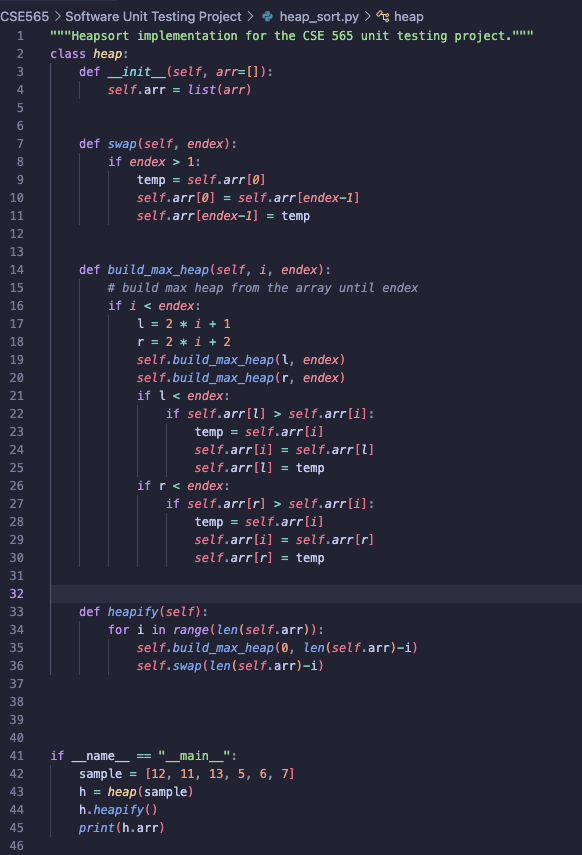
\includegraphics[width=0.7\linewidth]{screenshots/heap_sort.png}
\caption{Heapsort implementation shown in the development environment.}
\end{figure}

\section{Unit Testing Framework and AI Prompt Generation}

I used Python's built-in \texttt{unittest} framework. The Python documentation describes \texttt{unittest} as a unit testing framework that supports test automation, test fixtures, test cases, and grouping tests into collections (Python Software Foundation, n.d.-a). I chose this framework because it comes with Python, requires no additional packages, and supports clear assertions for comparing the expected and actual output of the Heapsort algorithm.

A generative AI tool was used to create the first version of the unit tests. The prompt explained
the interface of my implementation and asked the AI to generate tests for normal and edge-case
inputs.

\subsection{Prompt Used}

\begin{lstlisting}[style=code]
I wrote a Python Heapsort implementation for a software unit testing project.
The code defines a class named heap. To use it, create h = heap(input_list),
call h.heapify(), and then check h.arr for the sorted result.

Please generate Python unittest test cases for this Heapsort implementation.
Cover normal input and edge cases, including an empty list, one-element list,
already sorted list, reverse-sorted list, duplicate values, negative numbers,
mixed positive and negative numbers, and all equal values.
\end{lstlisting}

\begin{figure}[H]
\centering
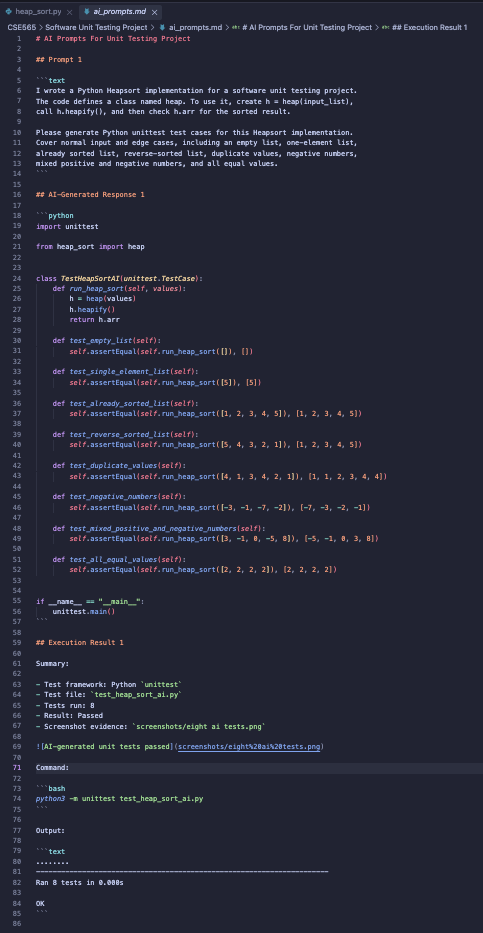
\includegraphics[width=0.6\linewidth]{screenshots/ai_prompt_response.png}
\caption{AI prompt and generated response used to create the first test suite.}
\end{figure}

\section{AI-Generated Test Cases}

The AI-generated unit tests were saved in \texttt{test\_heap\_sort\_ai.py}. The test file contains
eight tests covering empty input, a single-element list, an already sorted list, a reverse-sorted
list, duplicates, negative numbers, mixed positive and negative numbers, and all-equal values.

\subsection{AI-Generated Test Code}

\lstinputlisting[style=code,language=Python]{test_heap_sort_ai.py}

\section{AI-Generated Test Execution}

The AI-generated tests were executed with this command:

\begin{lstlisting}[style=code]
python3 -m unittest test_heap_sort_ai.py
\end{lstlisting}

The test run completed successfully.

\begin{itemize}
    \item Test framework: Python \texttt{unittest}
    \item Test file: \texttt{test\_heap\_sort\_ai.py}
    \item Tests run: 8
    \item Result: Passed
\end{itemize}

\begin{lstlisting}[style=code]
........
----------------------------------------------------------------------
Ran 8 tests in 0.000s

OK
\end{lstlisting}

\begin{figure}[H]
\centering
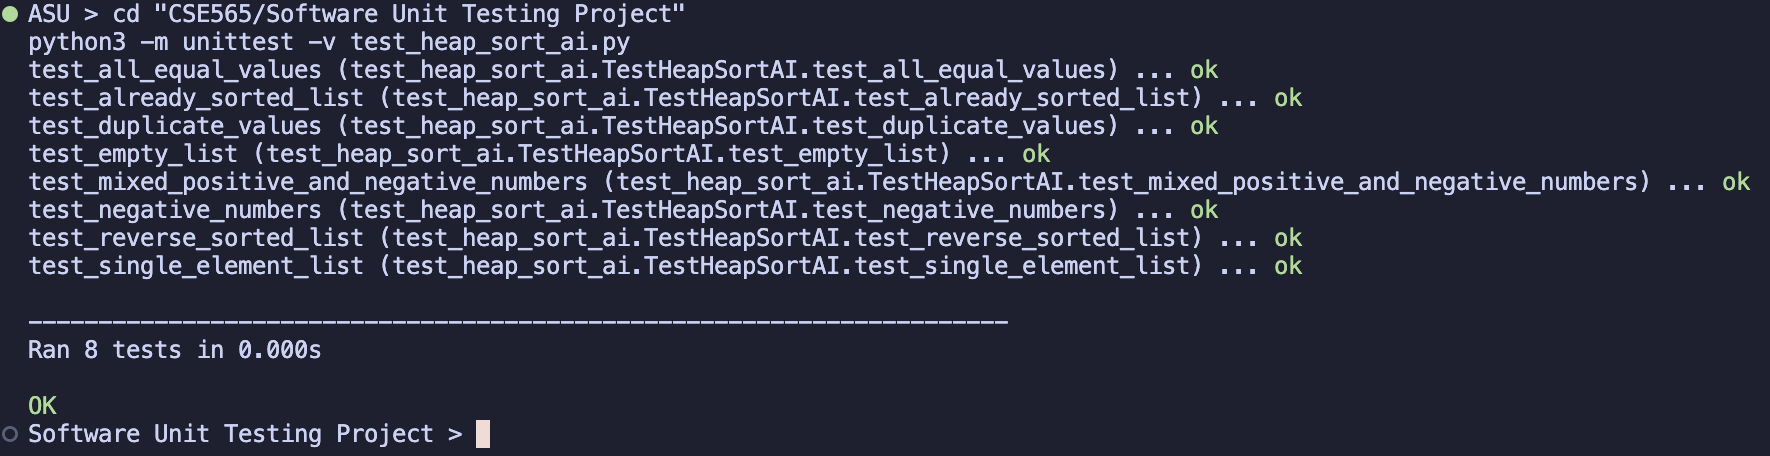
\includegraphics[width=0.95\linewidth]{screenshots/eight ai tests.png}
\caption{AI-generated unit tests passing.}
\end{figure}

\section{Assessment and Improvement of Test Cases}

The AI-generated tests were a good starting point because they tested several basic sorting cases.
However, the AI tests were mostly simple example-based tests. They did not check whether the
original input list stayed unchanged, did not use randomized testing, and did not compare many
different inputs against a trusted sorting function.

I improved the test suite in \texttt{test\_heap\_sort\_student.py}. The student-improved tests kept the original coverage and added stronger cases. Python's \texttt{sorted} function was useful as a comparison oracle because it returns a new sorted list from an iterable (Python Software Foundation, n.d.-b).

\begin{itemize}
    \item A test for preserving the original input list
    \item A larger reverse-sorted list
    \item Mixed float, negative, and duplicate values
    \item Randomized lists compared against Python's built-in \texttt{sorted} function
    \item The student-added float list and larger shuffled integer list tests
\end{itemize}

\subsection{Student-Improved Test Code}

\lstinputlisting[style=code,language=Python]{test_heap_sort_student.py}

\section{Student-Improved Test Execution}

The improved student tests were executed with this command:

\begin{lstlisting}[style=code]
python3 -m unittest -v test_heap_sort_student.py
\end{lstlisting}

The improved test run completed successfully.

\begin{itemize}
    \item Test framework: Python \texttt{unittest}
    \item Test file: \texttt{test\_heap\_sort\_student.py}
    \item Tests run: 14
    \item Result: Passed
\end{itemize}

\begin{lstlisting}[style=code]
test_all_equal_values ... ok
test_already_sorted_list ... ok
test_duplicate_values ... ok
test_empty_list ... ok
test_float_list ... ok
test_large_reverse_sorted_list ... ok
test_mixed_float_negative_and_duplicate_values ... ok
test_mixed_positive_and_negative_numbers ... ok
test_negative_numbers ... ok
test_original_input_is_not_changed ... ok
test_random_element_list ... ok
test_random_lists_match_python_sorted ... ok
test_reverse_sorted_list ... ok
test_single_element_list ... ok

----------------------------------------------------------------------
Ran 14 tests in 0.001s

OK
\end{lstlisting}

\begin{figure}[H]
\centering
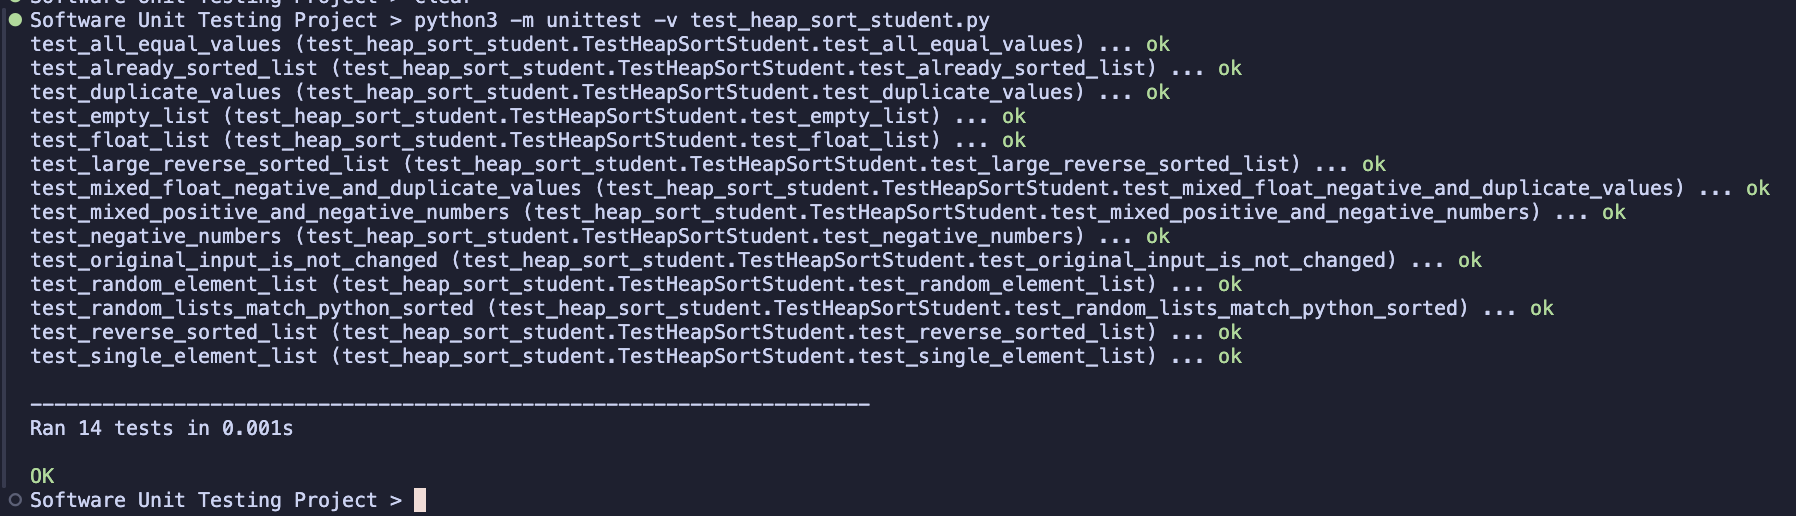
\includegraphics[width=0.95\linewidth]{screenshots/student added tests.png}
\caption{Student-improved unit tests passing.}
\end{figure}

\section{Assessment of the Generative AI Tool}

The generative AI tool was useful for quickly creating a baseline unit test suite. It understood
the interface of my Heapsort implementation, used the \texttt{unittest} framework correctly, and
created tests for common cases such as empty lists, duplicate values, negative numbers, and
reverse-sorted input.

The weakness of the AI-generated suite was that it did not go far beyond basic examples. It did
not test whether the original input list was preserved, did not use randomized testing, and did
not compare a variety of generated inputs against a known correct result. Because of that, human
review was still necessary.

Overall, the AI tool was effective as a starting point, but it did not replace the need for
student judgment. The AI-generated tests helped begin the testing process, while the
student-improved tests gave stronger confidence that the Heapsort implementation behaves
correctly.

\section{Conclusion}

This project implemented the Heapsort algorithm, generated unit tests using a generative AI tool,
executed the AI-generated tests, evaluated their strengths and weaknesses, and improved the test
suite with additional student-created cases. The AI-generated test suite passed all 8 tests, and
the student-improved test suite passed all 14 tests.

\section*{References}

\hangindent=0.5in Python Software Foundation. (n.d.-a). \textit{\texttt{unittest} --- Unit testing framework}. Python documentation. Retrieved August 29, 2026, from \url{https://docs.python.org/3/library/unittest.html}

\hangindent=0.5in Python Software Foundation. (n.d.-b). \textit{Sorting techniques}. Python documentation. Retrieved August 29, 2026, from \url{https://docs.python.org/3/howto/sorting.html}

\end{document}
